\begin{frame}
    \frametitle{Representación de pose en 2D}
    \footnotesize
    Modelamos el robot como un cuerpo rígido sobre ruedas, que opera en un plano horizontal. La dimensionalidad total de este chasis de robot en el plano es de tres, dos para la posición en el plano y uno para la orientación a lo largo del eje vertical, que es ortogonal al plano.

    \begin{figure}[!h]
        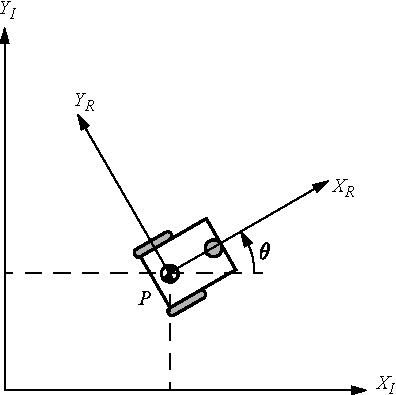
\includegraphics[width=0.4\columnwidth]{./images/coordinate_systems.pdf}
        \caption{El marco de referencia global y el marco de referencia local del robot.}
    \end{figure}

    Para especificar la posición del robot en el plano, establecemos una relación entre el marco de referencia global y el marco de referencia local del robot.

\end{frame}


\begin{frame}
    \frametitle{Representación de pose en 2D}
    \footnotesize
    
    \begin{center}
        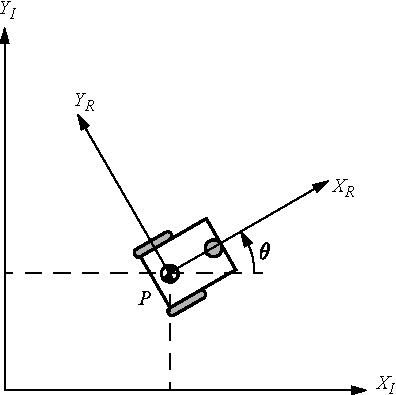
\includegraphics[width=0.4\columnwidth]{./images/coordinate_systems.pdf}
    \end{center}

    \note{Un marco de referencia inercial es un marco de referencia que no está experimentando aceleración. La física de un sistema en un marco inercial no tiene fuerzas externas al sistema.}
    
    \note{Ejemplo de sistema no inercial: una bola que cae hacia el suelo no va exactamente hacia abajo porque la Tierra está girando, lo que significa que el marco de referencia de un observador en la Tierra no es inercial. La física debe tener en cuenta el efecto Coriolis, en este caso considerado como una fuerza, para predecir el movimiento horizontal.}
    
    
    Para especificar la posición del robot, elegimos un punto $p$ en el chasis del robot como su punto de referencia de posición. La base $\left\lbrace X_R,Y_R \right\rbrace$ define dos ejes en relación con $p$ en el chasis del robot y, por lo tanto, es el marco de referencia local del robot. La posición de $p$ en el marco de referencia global se especifica mediante las coordenadas $x$ e $y$, y la diferencia angular entre los marcos de referencia global y local está dada por $\theta$.
    
    La pose del robot estará dada por la posición y la orientación:
    
    \begin{equation*}
        \xi_{I} = \begin{bmatrix}
            x\\
            y\\
            \theta
        \end{bmatrix}
    \end{equation*}
\end{frame}


\begin{frame}
    \frametitle{Representación de pose en 2D}
    \footnotesize
    
    \begin{center}
        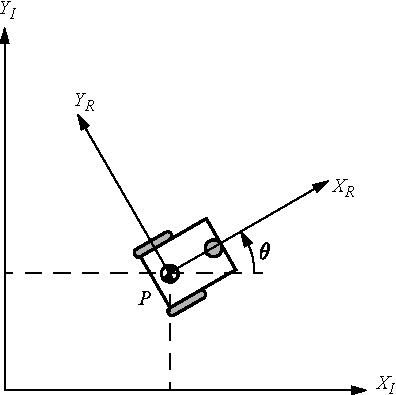
\includegraphics[width=0.4\columnwidth]{./images/coordinate_systems.pdf}
    \end{center}

    Esta matriz se puede utilizar para mapear el movimiento en el marco de referencia global ?? XI YI? al movimiento en términos del marco de referencia local ?? XR YR ?. Esta operación se denota por R? ()? ·

    \begin{equation*}
        R(\theta)=\begin{bmatrix}
            \cos\theta & \sin\theta & 0\\
            -\sin \theta & \cos \theta & 0\\
            0 & 0 & 1
        \end{bmatrix}
    \end{equation*}
    
    \begin{equation*}
        \dot{\xi_R} = R(\dfrac{\pi}{2}) \dot{\xi_I}
    \end{equation*}
    
    Dada alguna velocidad (??? · X · y ·) en el marco de referencia global, podemos calcular las componentes del movimiento a lo largo de los ejes locales XR y de este robot. En este caso, debido al ángulo YR específico del robot, el movimiento a lo largo de XR es igual a, y el movimiento a lo largo de YR es: y · –x ·
    
\end{frame}

\begin{frame}
    \frametitle{Right-hand rule}
    En Robótica la disposición de los ejes de coordenadas y el sentido de rotación de los mismos está dado por la regla de la mano derecha (Right-hand rule).
    
    \begin{figure}[!h]
        \centering
        \subfloat[]
        {
            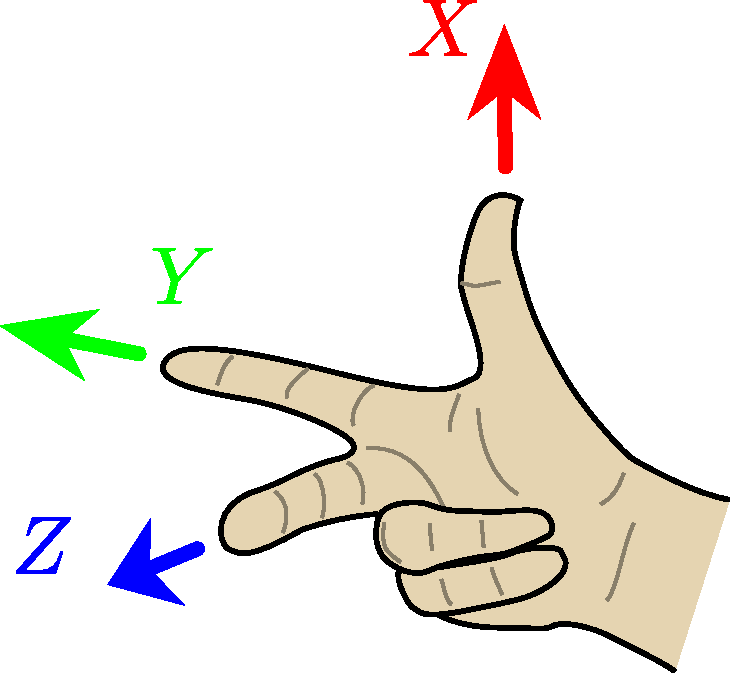
\includegraphics[width=0.4\columnwidth]{./images/right_hand_rule.pdf}
        }\hfill
        \subfloat[]
        {
            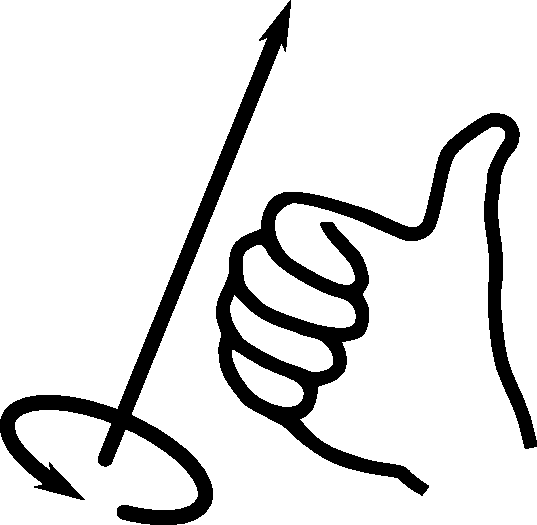
\includegraphics[width=0.4\columnwidth]{./images/right_hand_rule_positive_rotation.pdf}
        }
    \end{figure}
\end{frame}

\begin{frame}
    \frametitle{Roll Pitch Yaw }
        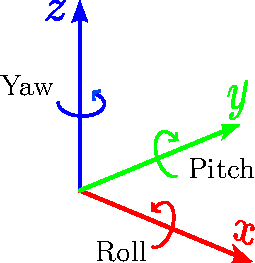
\includegraphics[width=0.5\columnwidth]{./images/roll_pitch_yaw.pdf}
        
        \TODO{Gimbal-Lock Video explanation: https://youtu.be/-WXfEPg8eMM}
\end{frame}
       
\begin{frame}
    \frametitle{Left-hand vs Right-hand rule}
    \begin{center}
        \only<1>{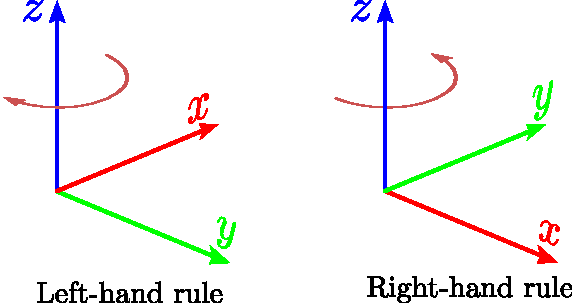
\includegraphics[width=\columnwidth]{./images/left_right_hand_rule.pdf}}
        \only<2>{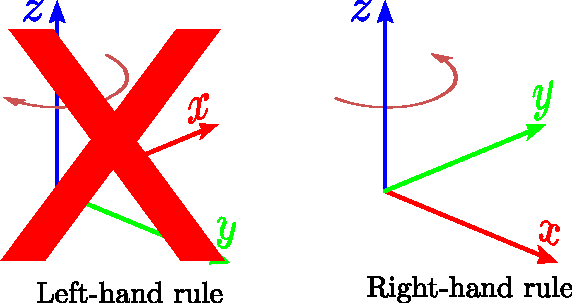
\includegraphics[width=\columnwidth]{./images/left_right_hand_rule_cross.pdf}}
    \end{center}
\end{frame}

\begin{frame}
    \frametitle{Formas de representar rotaciones}
    \TODO{Comentar euler, rotation matrix, pitch-yaw-roll y quaternions}
\end{frame}

